El sólido $E$ se obtiene al girar la región sombreada una vuelta completa alrededor del eje $z$. Evalúa
\[
\iiint_E (x^2+y^2+z^2)\,dV.
\]

\begingroup
\shorthandoff{>}
\begin{center}
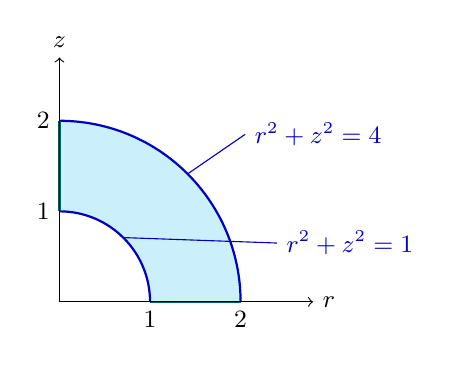
\begin{tikzpicture}[every node/.style={font=\small},scale=1.15]
    \fill[cyan!20] (0,2) arc[start angle=90,end angle=0,radius=2]
        -- (1,0) arc[start angle=0,end angle=90,radius=1] -- cycle;
    \draw[blue!75!black,thick] (0,2) arc[start angle=90,end angle=0,radius=2];
    \draw[blue!75!black,thick] (1,0) arc[start angle=0,end angle=90,radius=1];
    \draw[teal!75!black,thick] (0,1) -- (0,2) (1,0) -- (2,0);
    \draw[->] (0,0) -- (2.8,0) node[right] {$r$};
    \draw[->] (0,0) -- (0,2.7) node[above] {$z$};
    \node[left] at (0,1) {$1$};
    \node[left] at (0,2) {$2$};
    \node[below] at (1,0) {$1$};
    \node[below] at (2,0) {$2$};
    \draw[blue!75!black] (1.41,1.41) -- (2.05,1.85) node[right] {$r^2+z^2=4$};
    \draw[blue!75!black] (.71,.71) -- (2.4,.65) node[right] {$r^2+z^2=1$};
\end{tikzpicture}
\end{center}
\endgroup
